% ----------------------------------------------------------------
% Article Class (This is a LaTeX2e document)  ********************
% ----------------------------------------------------------------
\documentclass[12pt]{article}
\usepackage[english]{babel}
\usepackage{amsmath,amsthm}
\usepackage{graphicx}
\usepackage{amsfonts}
\usepackage{indentfirst}
\usepackage{lscape}
\usepackage[top=2.5cm,bottom=2.5cm,right=2.5cm,left=2.5cm]{geometry}
% THEOREMS -------------------------------------------------------
\newtheorem{thm}{Theorem}[section]
\newtheorem{cor}[thm]{Corollary}
\newtheorem{lem}[thm]{Lemma}
\newtheorem{prop}[thm]{Proposition}
\theoremstyle{definition}
\newtheorem{defn}[thm]{Definition}
\theoremstyle{remark}
\newtheorem{rem}[thm]{Remark}
\numberwithin{equation}{section}
% ----------------------------------------------------------------
\begin{document}
\title{User requirements}%
\author{Etienne Caillaud, Thomas Le Bris, Ibrahima Gueye, Gaetan Adier}%
\maketitle
\newpage

\tableofcontents
\newpage
% ----------------------------------------------------------------
\section{Context}
\subsection{Context and environment}
The project will take place in the XLIM-SIC laboratory of Poitiers University.

It will be about researching for new feature matching and indexing solutions by using new attributes including color and texture features. The final aim of the project will be the participation 
to the life CLEF contest 2015 which is a competition on the indexing of nature images.

\subsection{Aim of project}

The project is about identifying and indexing images. The aim is to obtain a new system for image indexing and recognition which is able to work on nature images (that is a huge problem for the standard descriptors which do not include texture or color features). We will have to develop a software program to test the effectiveness of many descriptors. Using this software program, we will be able to compare our results, with the new texture and color descriptors, to obtain the best results in the CLEF challenge.

This project is completely relevant to our training because it includes many subject as image processing and we will have to use many technologies (as Python or C++) to implement it.

There are many educational topics related to this project. We will have to work on project management, do some teamwork and use many image processing skills that we did not know before. We will have to report to our customer and it will be a good exercise for our future professional life.

\subsection{Scope of work}
We will have to design a software program which, by using the CLEF image learning Database, will be able to index the whole Database according to the different features which are specified in the CLEF rules.

The aim of this project is to adapt the last up to date designed texture and color attributes to the current image classification and then to measure how they perform with photographies taken from nature in order to test their competitiveness through the CLEF challenge.

The XLIM-SIC laboratory is currently working on the design of new image descriptors by integrating texture and color attributes more effectively. This project is a way for the researchers to see how they will behave in a real situation. Furthermore, the start of this project corresponds to the CLEF 2015 contest which is coincidentally about image recognition and automatic indexing of images taken from nature. If the results from this project are satisfying enough, they will be submitted to this international contest.

\subsection{Stakeholders}
\begin{itemize}
  \item Customer:
  Thierry Urruty.
  \item People involved in the project:
  Thomas Le Bris, Gaetan Adier, Ibrahima Gueye, Etienne Caillaud, David Helbert, Noel Richard.
  \item End users:
  Various image database structures (Flicker, Google, CIBDI Angouleme, Ainden...).
\end{itemize}
\subsection{State of the art}

The CLEF contest is a competition between many international laboratories. This competition began in 2010 so we can see what the other laboratories are doing nowadays.

We can see that all the competitors use SIFT or SURF descriptors. In the 2014 contest IBM was the laboratory which had the best results\cite{GOEAU2014}. After analysing what they do, we have concluded that they used all existing descriptors and mix them randomly.

After analysing the result of the 2014 contest we have agreed to use FINKI as a reference \cite{QUIANG2014}. FINKI uses segmentation and after then chooses between two descriptors (multiscale triangular shape or opponent SIFT).

\section{Constraints}
\subsection{Deadlines}

The finished product must be submitted by the 9th June 2015 including all necessary documentations.

The presentation will take place on the 15th June 2015.

SCRUM meetings will be scheduled every morning under the lead of Mr Chatellier.

Weekly meetings with tutors will be scheduled according to availabilities and needs

\section{Description of the final product}

A software program able to calculate a texture type descriptor suitable to nature images and which confirms the performances of this attribute via the CLEF contest results.

Locally, we will have to create one directory for each descriptor which will contain one CSV file in which we will find the descriptors. One text file will be created too and will contain all
the information about the image. To facilitate the indexing, one single text file will be created for the whole database and will contain all the information (image $\rightarrow$ descriptor 1
/ descriptor 2 / �) as an table of contents. Descriptors must be interchangeable in the software.

When this software program is finished to compute, we will have to compare our results with those of the other laboratories which have participated in the CLEF challenge. We will use the CLEF challenge metrics which are specified in the challenge rules.
An abstract of these comparisons will be provided with the software program and the final technical report.

\section{Organization and project management}
\subsection{Schedule}

List of tasks:
\begin{itemize}
  \item Writing the state of the art report
  \item Learning the use of HULK calculator
  \item Preparation of the database
  \subitem Constitution of database structure
  \subitem Calculation of SIFT descriptors
  \item Programming
  \subitem Programming $C_{2}O$ descriptor calculation
  \subitem Programming the distance calculation function
  \subitem Writing of the technical documentation
  \subitem Calculation of $C_{2}O$ descriptors
  \subitem Compare result using CLEF metrics
  \item Writing of final report
  \item Writing of oral presentation
\end{itemize}

cf. appendix A.

\subsection{Place}

The project will take place in the project classrooms (ON03/01/17) in the SP2MI building belonging to the University of Poitiers.

\section{Necessary resources for development}

List of necessary resources for development.

Connection to computing server of the university (HULK).

Computers with Python edition tools are the only necessity (can be found on the ones from the university).

The project participants will have to use their own computers, a place with electrical outlets and Internet access will be sufficient.



%-------------------Bibliography----------------------------------
\bibliographystyle{plain}
\bibliography{User_requirements}
% ----------------------------------------------------------------


%-----------------------------------------------------------------
%-------------------ANNEXES---------------------------------------
\newpage
\appendix

\begin{landscape}
\section{Gantt chart}
\begin{figure}[h]
  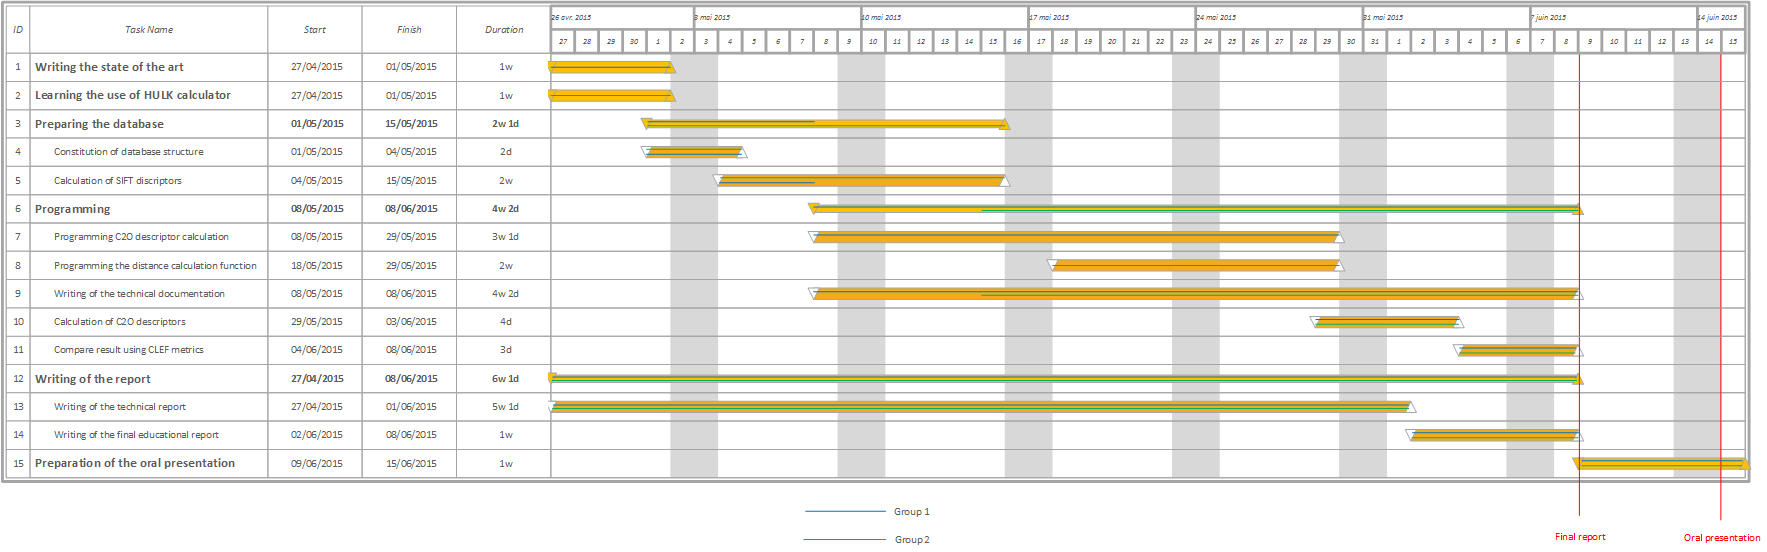
\includegraphics[scale=0.50]{Diagramme_de_Gantt.png}
  \caption{Gantt chart}\label{chart 1}
\end{figure}
\end{landscape}
% ----------------------------------------------------------------
\end{document}